% XADD Approximation
Recently, symbolic dynamic programming (SDP) ~\cite{sanner_uai11} have provided exact solutions for mixed discrete and continuous (hybrid) MDPs with piecewise linear dynamics and continuous actions\cite{zamani12}. The use of symbolic representation for functions in planning requires an efficient representation of dependencies, therefore an appropriate data structure was necessary. So this recent works provided a gain in compactness by extending Decision Diagrams to represent symbolic piecewise functions, creating the extended algebraic decision diagram (XADD). Using XADDs for efficient storage and manipulation of case based functions SDP methods have been able to solve problems such as multivariate inventory control for which exact solutions were previously considered intractable. Nevertheless, case representation and the symbolic XADD-based solutions are still quite sensitive to increase in the problem size, which can generally lead to exponential number of partitions. This lead for the motivating question of this work, whether XADDs efficiently compressed by approximation within fixed error bounds.

 A natural example of a piecewise linear function that can be approximated very efficiently is a regular difference step function, as the one in picture \ref{fig:stepf}. For this function it seems clear that with a small error, in this particular case, independent of the number of partitions, a much simpler representation can be achieved by modifying the linear function and merging the regions. We would like to represent it in a single partition as in figure \ref{fig:steptolin}. So our problem became of how automatically discovering appropriate linear functions that can replace the original functions in more than one partition while incurring minimal error. It is important to note that our merging strategy involves calculating a new linear function, that can optimally approximate the two previous linear functions in their corresponding regions but may be of a reasonably distinct kind, for instance it may not be obtainable as a linear combination of the original case functions.
 
The problem we discovered turned to be a piecewise bilinear saddle optimization, and a original solution for specific optimization problem was proposed. The solution involves a dual stage iterative algorithm that requires solutions of linear programs with an increasing number of constraints to obtain the optimal solution for the bilinear problem. This solution permits
the use of efficient linear program solvers and enables a novel class
of bounded approximate SDP algorithms based on XADD compression.

The gain in efficiency allows solution of many larger problems where exact SDP would be intractable. Moreover, this algorithm performs approximation with bounded error guarantees which is another innovattion for Hybrid MDP solutions.

\begin{figure}[!ht]
\centering
\begin{minipage}{.3\textwidth}
  \centering
  \subfigure[Step function] {
	\fbox{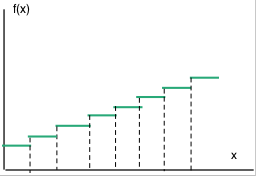
\includegraphics[scale=0.5]{Figures/stepfun/step.png}}
	\label{fig:stepf}
  }
\end{minipage}
\begin{minipage}{.3\textwidth}
\centering
\subfigure[Linear Approximation] {
	 \fbox{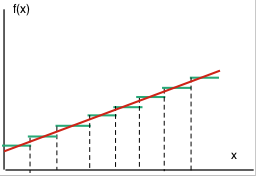
\includegraphics[scale=0.5]{Figures/stepfun/steplin.png}}
	\label{fig:steptolin} 
}
\end{minipage}
\caption{A step function can be much more compactly represented by a line that spans all partitions}
 \label{steppair1}
\end{figure}
